\documentclass[]{article}
\usepackage{geometry}
\geometry{
	a4paper,
	total={170mm,257mm},
	left=0.75in,
	top=0.75in,
	right=0.75in,
	bottom=1in,
}
\usepackage{gensymb}
\usepackage{lipsum}
\usepackage{graphicx}
\usepackage{amsmath}
\usepackage{xcolor}
\usepackage[
  colorlinks,
  breaklinks,
  unicode
]{hyperref}
\newcommand\Colorhref[3][blue]{\href{#2}{\color{#1}#3}}
\title{\textbf{Beginner's guide to Basilisks}}
\author{Vatsal Sanjay\\vatsalsanjay@gmail.com}
\begin{document}
\maketitle
\begin{abstract}
This document is a review and guide to the installation and working of Basilisk \Colorhref{http://basilisk.fr/}{(link)}, written by St\'ephane Popinet and his group. These notes are for personal use only, and detailed guide could be found at \Colorhref{http://basilisk.fr/Tutorial}{$<$link$>$}.\\\par 
Regarding this file: Since basilisk is still in the early stages of development, the facts written in this document are subject to change. If you find any information here outdated or incomplete, please let me know. You can also clone this repository (\Colorhref{https://github.com/VatsalSy/GuideBasilisk}{https://github.com/VatsalSy/GuideBasilisk}), make changes and push it.
\end{abstract}
\section{Installing Basilisk}
Installation is quite easy. There are two ways: Using darcs OR using tarball. I prefer the first one (darcs) because it allows to easily pull any update that occurs in Basilisk. The steps of this section are taken from \Colorhref{http://basilisk.fr/src/INSTALL}{http://basilisk.fr/src/INSTALL}. They are self-explanatory I have included them here, just for the sake of completion. 
\subsection{Installing darcs (if unavailable)}
{\color{red}vatsal@cloneMachine:$\sim\$$} sudo apt-get install darcs flex make
\subsection{Some important side packages}
{\color{red}vatsal@cloneMachine:$\sim\$$} sudo apt-get install gnuplot imagemagick libav-tools smpeg-plaympeg graphviz valgrind gifsicle
\subsection{Getting Basilisk source code}
{\color{red}vatsal@cloneMachine:$\sim\$$} darcs get http://basilisk.fr/basilisk
\begin{figure}[h]
\centering
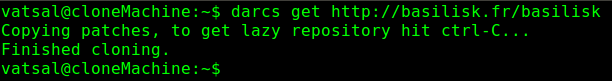
\includegraphics[width=0.75\linewidth]{Figure1}
\end{figure}
\paragraph{\textbf{Note:}} In order to pull new changes made in Basilisk, use:\\
{\color{red}vatsal@cloneMachine:$\sim\$$} cd basilisk\\
{\color{red}vatsal@cloneMachine:$\sim\$$} darcs pull\\
Then recompile.
\subsection{Compiling/recompiling Basilisk}
{\color{red}vatsal@cloneMachine:$\sim\$$} cd basilisk/src\\
{\color{red}vatsal@cloneMachine:$\sim\$$} export BASILISK=\$PWD\\
{\color{red}vatsal@cloneMachine:$\sim\$$} export PATH=\$PATH:\$PWD\\
{\color{red}vatsal@cloneMachine:$\sim\$$} ln -s config.gcc config\\
{\color{red}vatsal@cloneMachine:$\sim\$$} make -k\\
{\color{red}vatsal@cloneMachine:$\sim\$$} make

\section{Basilisk-View}
Details of bview: \Colorhref{http://basilisk.fr/src/README\#interactive-basilisk-view}{http://basilisk.fr/src/README\#interactive-basilisk-view}\\
Basilisk-view is similar to GfsView, with some minor differences:
\begin{enumerate}
\item Unlike GfsView, we cannot run bview on the fly while basilisk is running. We can, however, use it to render pictures and videos on the fly with bview. It can be used to look at the results after simulation is over, provided we have saved the intermediate files.
\item There is no program written analogous to gfs2oogl for bview. This means that we cannot interpolate the octree based data using available libraries. We could write our own code for it in future, something similar to gfs2oogl.
\item The coordinate systems for GfsView and Basilisk are different. GfsView output is rotated counter-clockwise compared to Gerris: this is due to the new N-ordering of quadtree cells (rather than 
Z-ordering). See these \Colorhref{https://groups.google.com/forum/\#!topic/basilisk-fr/yGedVYOCz8E}{link1} and \Colorhref{https://groups.google.com/forum/\#!topic/basilisk-fr/A6TKu16wbsQ}{link2}.
\item I found a working example for tecplot users \Colorhref{http://basilisk.fr/sandbox/hiroumi/tecplot/}{(here)}, but I have not tested it yet. 
\end{enumerate}
GfsView can still be used with Basilisk, provided that the code does not use \textquotedblleft mask\textquotedblright command. Mask command is used for creating solid objects and non-square (non-cubical) geometries. The precursor to using gfsview and writing \textquotedblleft.gfs\textquotedblright files, \textquotedblleft dump\textquotedblright is not compatible with \textquotedblleft mask\textquotedblright. Most likely, even bview cannot be used to look at intermediate files when \textquotedblleft mask\textquotedblright is used, but I have not changed it. For other compatibility issues, visit: \Colorhref{http://basilisk.fr/src/COMPATIBILITY}{http://basilisk.fr/src/COMPATIBILITY}.
\subsection{Installing bview}
Sources: (go in this order)
\begin{enumerate}
\item bview: \Colorhref{http://basilisk.fr/src/bview}{http://basilisk.fr/src/bview}
\item Screen rendering: \Colorhref{http://basilisk.fr/src/gl/INSTALL}{http://basilisk.fr/src/gl/INSTALL}
\item Python for bview-client: \Colorhref{http://basilisk.fr/src/bview-client.py}{http://basilisk.fr/src/bview-client.py}
\item Actual installation: \Colorhref{http://basilisk.fr/src/bview-server.c}{http://basilisk.fr/src/bview-server.c}
\end{enumerate}
\subsubsection{Dependencies}
For cluster for off-screen rendering:\\
{\color{red}vatsal@cloneMachine:$\sim\$$} sudo apt-get install libglu1-mesa-dev libosmesa6-dev\\
{\color{red}vatsal@cloneMachine:$\sim\$$} cd \$BASILISK/gl\\
{\color{red}vatsal@cloneMachine:$\sim\$$} make libglutils.a libfb\_osmesa.a\\
Another method would be to use the following (recommended for laptops), the above dependencies are recommended for clusters.\\
{\color{red}vatsal@cloneMachine:$\sim\$$} sudo apt-get install libglu1-mesa-dev libglew-dev libgl1-mesa-dev\\
{\color{red}vatsal@cloneMachine:$\sim\$$} cd \$BASILISK/gl\\
{\color{red}vatsal@cloneMachine:$\sim\$$} make libglutils.a libfb\_glx.a\\
The following is required for both the above versions:\\
{\color{red}vatsal@cloneMachine:$\sim\$$} sudo apt-get install python-pil.imagetk
\subsubsection{bview}
\textbf{(Optional)} Add this line at the end of config.gcc, depending on the type of machine and dependency selected:\\
Osmesa (Cluster):
\begin{verbatim}[frame=singhe]
OPENGLIBS = -lfb_osmesa -lGLU -lOSMesa
\end{verbatim}
Glx (Laptop):
\begin{verbatim}
OPENGLIBS = -lfb_glx -lGLU -lGLEW -lGL -lX11
\end{verbatim}
Then do this:\\
{\color{red}vatsal@cloneMachine:$\sim\$$} cd \$BASILISK\\
{\color{red}vatsal@cloneMachine:$\sim\$$} make bview-servers\\
For a typical bview use and environment, follow the example at:\Colorhref{http://basilisk.fr/src/bview}{http://basilisk.fr/src/bview}
\section{A typical code}
Basilisk codes are modified C++ files.\\
A good place to start understanding Basilisk would be \Colorhref{http://basilisk.fr/Tutorial}{http://basilisk.fr/Tutorial}. Here, I have added the case of liquid jet atomization. I have tried to compare and contrast this case with the famous jet atomization case simulated using gerris (which we are more familiar with).\\
\subsection{Header File}
Just like a standard C++ code, we need to include the libraries that we are going to use.
\begin{verbatim}
#include "navier-stokes/centered.h"
#include "two-phase.h"
#include "tension.h"
#include "tag.h"
#include "view.h"
\end{verbatim}
\begin{enumerate}
\item \Colorhref{http://basilisk.fr/src/navier-stokes/centered.h}{\textit{navier-stokes/centered.h}} is the normal Gerris implemented Navier-Stokes equation solver for incompressible variable (two-phase) density flow.
\item \Colorhref{http://basilisk.fr/src/two-phase.h}{\textit{two-phase.h}} is the simulations setup file for flows of two fluids separated by an interface (i.e. immiscible fluids). It is typically used in combination with a Navier–Stokes solver.
\item \Colorhref{http://basilisk.fr/src/tension.h}{\textit{tension.h}} includes the surface tension force, same as Gerris by adding $\sigma\kappa\delta_i$ term in NS equation.
\item \Colorhref{http://basilisk.fr/src/tag.h}{\textit{tag.h}} is used to count the number of droplets in the simulation. Unlike Gerris, in Basilisk, we get this special feature which when combined with a small sub-routine (given later) can count the number of droplets.
\item \Colorhref{http://basilisk.fr/src/view.h}{\textit{view.h}} is important for using Basilisk-View. 
\end{enumerate}
\subsection{Defining custom variables}
\begin{verbatim}
#define radius 1./12.
#define length 0.025
#define Re 5800
#define SIGMA 3e-5
int maxlevel = 7;
double uemax = 0.1;
\end{verbatim}
Just like Gerris, here we can define some global variables which can be used later on in the file. For this specific example, radius is the radius of the liquid jet, length is the initialized length (similar to Gerris, we will initialize a small length of the jet and highly refine that part at t = 0), $Re$ is the Reynold's number of the liquid jet, SIGMA is the $\sigma$ (surface tension) at liquid-air interface, maxlevel is the maximum octree refinement level and uemax is the maximum allowable error in the velocity field.
\subsection{Initial Conditions}
\begin{verbatim}
scalar f0[];
//Initial conditions
event init (t = 0) {
  if (!restore (file = "dump")) {
    refine (x < 1.2*length && sq(y) + sq(z) < 2.*sq(radius) && level < maxlevel);
    fraction (f0, sq(radius) - sq(y) - sq(z));
    f0.refine = f0.prolongation = fraction_refine;
    restriction ({f0});
    foreach() {
      f[] = f0[]*(x < length);
      u.x[] = f[];
    }
    boundary ({f,u.x});
  }
}
\end{verbatim}
A scalar field $f0$ is defined. It is analogous to the $T0$ variable we usually define in Gerris. An event instance is declared for declaring initial conditions. The commands are executed if and only if the file named \textquotedblleft dump\textquotedblright is not present. The grid is refined in a cylindrical region, 1.2 times the size of initialized jet and $\sqrt{2}$ times its radius. Further, the variable field $f0$ is set at 1 inside the cylinder ($y^2 + z^2 < r^2$) and zero otherwise. Moreover, \textit{f0.refine = f0.prolongation = fraction\_refine;} refines the volume fraction field (\Colorhref{http://basilisk.fr/src/fractions.h\#32}{details}). Further, \textit{restriction({f0});} is used for boundary conditions on levels. The \textit{foreach} command is a modified \textit{for} loop to initialize the initial conditions in all the cells. At last, \textit{boundary ({f,u.x});} defines the boundary conditions at t = 0 (\Colorhref{http://basilisk.fr/Basilisk\%20C\#boundary-conditions}{details}). The stencils located near the boundary extends beyond it and the last line initializes these ghost values. By default, the boundary condition is symmetry and if the domain values are modified, it is necessary to modify the ghost values as well and therefore the last line is needed. 
\subsection{Boundary Condition}
\begin{verbatim}
/* We then set an oscillating inflow velocity on the
left-hand-side and free outflow on the right-hand-side. */
u.n[left]  = dirichlet(f0[]*(1. + 0.05*sin (10.*2.*pi*t)));
u.t[left]  = dirichlet(0);
p[left]    = neumann(0);
f[left]    = f0[];
u.n[right] = neumann(0);
p[right]   = dirichlet(0);
\end{verbatim}
Setting boundary conditions is intuitive and the above code snip is self-explanatory. Unlike Gerris, we do not have to create the web of boxes and manually see to the inter-connectivities. In order to get a cuboidal (rectangular) domain or create complex geometries, \textquotedblleft mask\textquotedblright can be used. However, \textquotedblleft dump\textquotedblright command used to write output data is not compatible with \textquotedblleft mask\textquotedblright yet. 
\subsection{Adaptive Mesh Refinement}
\begin{verbatim}
event adapt (i++) {
  adapt_wavelet ({f,u}, (double[]){0.01,uemax,uemax,uemax}, maxlevel);
}
\end{verbatim}
Basilisk uses the \textquotedblleft wavelet\textquotedblright method for AMR based on the maximum allowable error. In the syntax, \textit{\{f,u\}} defines the variables based on which refinement is to be done (please note, it is a 4 element vector). In the second term, \text{\{{0.01,uemax,uemax,uemax}\}} enlists the maximum error allowed. 
\subsection{The end time of simulation}
Unlike Gerris, there is no option to set end-time in Basilisk (that I could find). It is set with the maximum time event available in the script. Therefore, we can make one event to be executed at the end time of simulation and do not mention time anywhere else in the code. Please note that the \textquotedblleft event\textquotedblright is 
\begin{verbatim}
event end (t = 2.5) {
  printf ("i = %d t = %g\n", i, t);
}
\end{verbatim}
\subsection{The main run snippet}
\begin{verbatim}
int main ()
{
  /**
  The initial domain is discretised with $64^3$ grid points. We set
  the origin and domain size. */
  init_grid (64);
  origin (0, -1.5, -1.5);
  L0 = 3.;
  /*
  We set the density and viscosity of each phase as well as the
  surface tension coefficient and start the simulation. */
  rho1 = 1., rho2 = 1./27.84;
  mu1 = 2.*radius/Re*rho1, mu2 = 2.*radius/Re*rho2;
  f.sigma = SIGMA;
  run();
}
\end{verbatim}
This is the main function which executes the simulation. The command \textit{init\_grid (n)} descritizes the domain length in n number of cells. \\
\paragraph{\textbf{Origin:}} Setting origin is different than that in Gerris. Origin can be set using \textit{origin ($x_0$, $y_0$, $z_0$)}. In this, ($x_0$, $y_0$, $z_0$) is the co-ordinate location of the left-bottom-back corner with respect to the intended origin. For example, if you want the origin to be at center of the left wall, the command will read (0, -1.5, -1.5).\\
\textit{L0} is used to set the length of the domain. Please note that the domain is always cubical in Basilisk. So if you want to make a cuboid then it is necessary to use \textquotedblleft mask\textquotedblright. The other variables, \textit{mi} and \textit{rhoi} ($\forall\:\:i \in \{1, 2\}$) define the viscosity and density respectively and are local variables to the file \textquotedblleft twophase.h\textquotedblright. At last, \textit{f.sigma} is the surface tension for the VOF tracer \textit{f}.
\subsection{Writing log files and on terminal}
\begin{verbatim}
event logWriting (i++) {
  static FILE * fp;
  if (i == 0) {
    fprintf (ferr, "i dt t\n");
    fp = fopen ("log", "w");
    fprintf (fp, "i dt t\n");
    fprintf (fp, "%d %g %g\n", i, dt, t);
    fclose(fp);
  } else {
    fp = fopen ("log", "a");
    fprintf (fp, "%d %g %g\n", i, dt, t);
    fclose(fp);
  }
  fprintf (ferr, "%d %g %g\n", i, dt, t);
}
\end{verbatim}
This part is used to output the simulation temporal information on the terminal as well as store them in the file named \textquotedblleft log\textquotedblright.
\subsection{Generating movies}
\begin{verbatim}
/**
We generate an animation using Basilisk View. */
event movie (t += 1e-2)
{
#if dimension == 2
  scalar omega[];
  vorticity (u, omega);
  view (tx = -0.5);
  clear();
  draw_vof ("f");
  squares ("omega", linear = true, spread = 10);
  box ();
#else // 3D
  scalar pid[];
  foreach()
    pid[] = fmod(pid()*(npe() + 37), npe());
  boundary ({pid}); // not used for the moment
  view (camera = "iso",
	fov = 14.5, tx = -0.418, ty = 0.288,
	width = 1600, height = 1200);
  clear();
  draw_vof ("f");
  box ();
#endif // 3D
  static FILE * fp = popen ("ppm2mp4 > movie.mp4", "w");
  save (fp = fp);
}
\end{verbatim}
This is just a typical code to generate movie of the simulation. For details, look at the guide to bview.
\subsection{Data dumping}
\begin{verbatim}
event snapshot (t = 0; t += 0.1)
{
  dump (file = "dump");
  char nameGfs[80];
  sprintf (nameGfs, "intermediateGfs/snapshot-%2.1f.gfs", t);
  output_gfs (file = nameGfs, t = t);
  char nameBview[80];
  sprintf (nameBview, "intermediateBview/snapshot-%2.1f", t);
  dump (file = nameBview);
}
\end{verbatim}
These are used to write data files. To write \textquotedblleft.gfs\textquotedblright files, \textit{output\_gfs (file = nameGfs, t = t);} is used. For writing data files read and processed by bview, \textquotedblleft dump (file = nameBview);\textquoteright can be used.
\subsection{Visualization on the fly}
Currently, bview is not equipped for visualization on the fly. But, the following code can be used to run gfsview on the go. 
\begin{verbatim}
event gfsview (i++) {
  static FILE * fp = popen ("gfsview3D", "w");
  output_gfs (fp);
}
\end{verbatim}
Please note that in presence of \textquotedblleft mask\textquotedblright, the \textquotedblleft dump\textquotedblright and \textquotedblleft output\_gfs\textquotedblright commands will write corrupted intermediate files.
\subsection{Running scripts}
\subsubsection{At t = 0}
To start the simulation, use the script file, named \textquotedblleft run0.sh\textquotedblright. It deletes the log and dump files if they exist and creates the empty folders. 
\begin{verbatim}
if [ -f "log" ];
then
rm log
fi

if [ -f "dump" ];
then
rm dump
fi

if [ -d "intermediateGfs" ]
then
rm -r intermediateGfs
fi

if [ -d "intermediateBview" ]
then
rm -r intermediateBview
fi

mkdir intermediateGfs
mkdir intermediateBview

qcc -O2 -Wall -grid=octree $file.c -o $file -lm \
    -L$BASILISK/gl -lglutils -lfb_glx -lGLU -lGLEW -lGL -lX11 -lm

#qcc -O2 -Wall $file.c -o $file -lm \
#    -L$BASILISK/gl -lglutils -lfb_osmesa -lGLU -lOSMesa -lm
\end{verbatim}
Moreover, in order to make changes in between the simulation and re-start it, the script file named \textquotedblleft runRe.sh\textquotedblright can be used. This simply compiles the code. 
\begin{verbatim}
if [ ! -d "intermediateGfs" ]
then
mkdir intermediateGfs
fi

if [ ! -d "intermediateBview" ]
then
mkdir intermediateBview
fi

qcc -O2 -Wall -grid=octree $file.c -o $file -lm \
    -L$BASILISK/gl -lglutils -lfb_glx -lGLU -lGLEW -lGL -lX11 -lm

#qcc -O2 -Wall $file.c -o $file -lm \
#    -L$BASILISK/gl -lglutils -lfb_osmesa -lGLU -lOSMesa -lm
\end{verbatim}
\end{document}
